\documentclass[tikz,border=8pt]{standalone}
% Shared look for every TikZ diagram. Load with % Shared look for every TikZ diagram. Load with % Shared look for every TikZ diagram. Load with \input{../../tools/tikz-style.tex}
\usepackage[T1]{fontenc}
\usepackage{lmodern}
\renewcommand{\sfdefault}{lmr}  % diagrams use the same serif as the text
\usetikzlibrary{arrows.meta, positioning, shapes.geometric, calc, fit, backgrounds}
\definecolor{cblue}{HTML}{4C78A8}
\definecolor{corange}{HTML}{F58518}
\definecolor{cgreen}{HTML}{54A24B}
\definecolor{cred}{HTML}{E45756}
\definecolor{cpurple}{HTML}{B279A2}
\definecolor{cgrey}{HTML}{6B6B6B}
\tikzset{
  every picture/.style={font=\sffamily, line width=1.2pt},
  box/.style={draw=#1, fill=#1!12, rounded corners=4pt, align=center, inner sep=7pt, minimum height=1.1cm},
  box/.default=cgrey,
  arrow/.style={-{Stealth[length=3mm]}, draw=cgrey, line width=1.4pt},
  title/.style={font=\sffamily\bfseries\Large},
  note/.style={font=\sffamily\small, text=cgrey, align=center},
}
\AtBeginDocument{\hyphenpenalty=10000 \exhyphenpenalty=10000}

\usepackage[T1]{fontenc}
\usepackage{lmodern}
\renewcommand{\sfdefault}{lmr}  % diagrams use the same serif as the text
\usetikzlibrary{arrows.meta, positioning, shapes.geometric, calc, fit, backgrounds}
\definecolor{cblue}{HTML}{4C78A8}
\definecolor{corange}{HTML}{F58518}
\definecolor{cgreen}{HTML}{54A24B}
\definecolor{cred}{HTML}{E45756}
\definecolor{cpurple}{HTML}{B279A2}
\definecolor{cgrey}{HTML}{6B6B6B}
\tikzset{
  every picture/.style={font=\sffamily, line width=1.2pt},
  box/.style={draw=#1, fill=#1!12, rounded corners=4pt, align=center, inner sep=7pt, minimum height=1.1cm},
  box/.default=cgrey,
  arrow/.style={-{Stealth[length=3mm]}, draw=cgrey, line width=1.4pt},
  title/.style={font=\sffamily\bfseries\Large},
  note/.style={font=\sffamily\small, text=cgrey, align=center},
}
\AtBeginDocument{\hyphenpenalty=10000 \exhyphenpenalty=10000}

\usepackage[T1]{fontenc}
\usepackage{lmodern}
\renewcommand{\sfdefault}{lmr}  % diagrams use the same serif as the text
\usetikzlibrary{arrows.meta, positioning, shapes.geometric, calc, fit, backgrounds}
\definecolor{cblue}{HTML}{4C78A8}
\definecolor{corange}{HTML}{F58518}
\definecolor{cgreen}{HTML}{54A24B}
\definecolor{cred}{HTML}{E45756}
\definecolor{cpurple}{HTML}{B279A2}
\definecolor{cgrey}{HTML}{6B6B6B}
\tikzset{
  every picture/.style={font=\sffamily, line width=1.2pt},
  box/.style={draw=#1, fill=#1!12, rounded corners=4pt, align=center, inner sep=7pt, minimum height=1.1cm},
  box/.default=cgrey,
  arrow/.style={-{Stealth[length=3mm]}, draw=cgrey, line width=1.4pt},
  title/.style={font=\sffamily\bfseries\Large},
  note/.style={font=\sffamily\small, text=cgrey, align=center},
}
\AtBeginDocument{\hyphenpenalty=10000 \exhyphenpenalty=10000}

\begin{document}
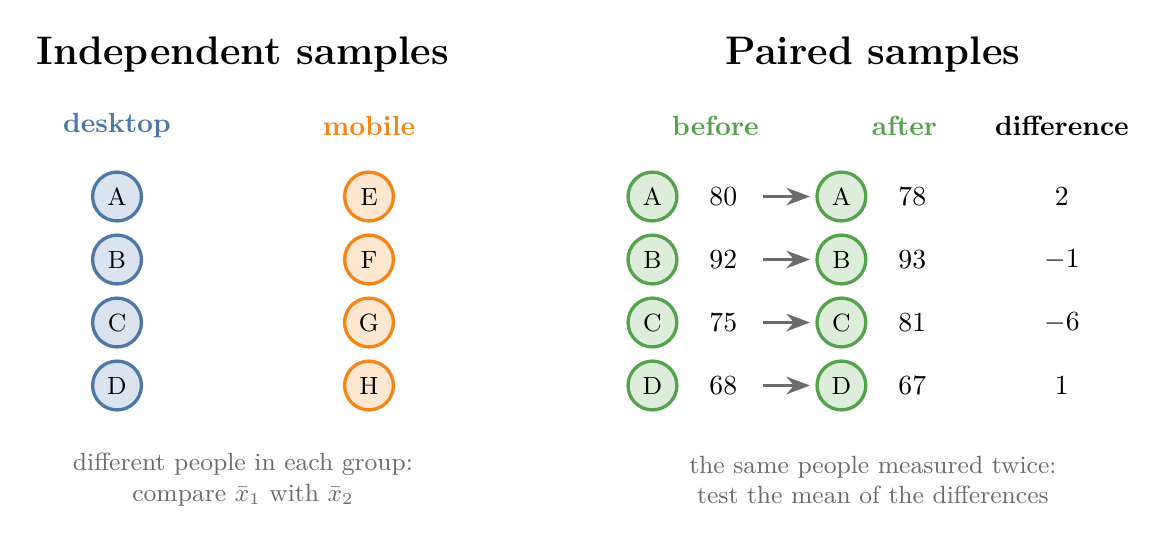
\begin{tikzpicture}
  \tikzset{p/.style={circle, draw=#1, fill=#1!20, minimum size=0.62cm, inner sep=0pt, font=\sffamily\small}}
  % independent design
  \node[title] at (0,1.2) {Independent samples};
  \node[font=\sffamily\bfseries, text=cblue] at (-1.6,0.3) {desktop};
  \node[font=\sffamily\bfseries, text=corange] at (1.6,0.3) {mobile};
  \foreach \i/\l in {0/A,1/B,2/C,3/D} \node[p=cblue] at (-1.6,-0.6-0.8*\i) {\l};
  \foreach \i/\l in {0/E,1/F,2/G,3/H} \node[p=corange] at (1.6,-0.6-0.8*\i) {\l};
  \node[note, align=center] at (0,-4.2) {different people in each group:\\ compare $\bar{x}_1$ with $\bar{x}_2$};
  % paired design
  \begin{scope}[xshift=8cm]
    \node[title] at (0,1.2) {Paired samples};
    \node[font=\sffamily\bfseries, text=cgreen] at (-2,0.3) {before};
    \node[font=\sffamily\bfseries, text=cgreen] at (0.4,0.3) {after};
    \node[font=\sffamily\bfseries] at (2.4,0.3) {difference};
    \foreach \i/\l/\b/\a in {0/A/80/78, 1/B/92/93, 2/C/75/81, 3/D/68/67} {
      \node[p=cgreen] (b\i) at (-2.8,-0.6-0.8*\i) {\l};
      \node at (-1.9,-0.6-0.8*\i) {\b};
      \node[p=cgreen] (a\i) at (-0.4,-0.6-0.8*\i) {\l};
      \node at (0.5,-0.6-0.8*\i) {\a};
      \draw[arrow, line width=1pt] (-1.4,-0.6-0.8*\i) -- (-0.8,-0.6-0.8*\i);
      \pgfmathtruncatemacro{\d}{\b-\a}
      \node at (2.4,-0.6-0.8*\i) {$\d$};
    }
    \node[note, align=center] at (0,-4.2) {the same people measured twice:\\ test the mean of the differences};
  \end{scope}
\end{tikzpicture}
\end{document}
